
\chapter{Toward Congruence}  

%Key pieces
%\begin{itemize}
%\item Transformations and symmetries
%\item Congruence via isometries
%\item Parity of isometries
%\item 1166 parallel postulate
%\item Similarity via dilations
%\end{itemize}

\section{Transformations, Symmetry, and Congruence}
In school mathematics, transformations and symmetry have typically been small niche topics, separate from each other, separate from most of the rest of school mathematics, and receiving little curricular attention.  Congruence, on the other hand, is a more prominent idea that begins informally in the elementary grades as ``same shape, same size'' and culminates in high school with axioms, theorems, and proofs.  

In this section, we demonstrate how transformations can undergird both symmetry and congruence, thereby strengthening all three topics and also establishing groundwork for an analogous approach to similarity.  

\subsection{Transformations}
Informally, a transformation of the plane is a ``motion,'' such as a rotation or a stretch of the plane.  More formally, a transformation is a function that takes points in the plane as inputs and gives points as outputs.\standardhs{G-CO.2}  In school mathematics, we consider only transformations that take lines to lines, so that key geometric features are ``preserved.''  For example a triangle remains a triangle when it is rotated and even when it is stretched.  

Transformations are often specified using a coordinate system, but coordinates are not necessary.  For now, we will explore transformations without a coordinate system.  Later, we will use coordinates, along with matrices and vectors, to describe transformations.  

\begin{definition}
Transformations that preserve distances and angles are called \emph{isometries}, and the most important of these are \emph{basic rigid motions}: translations, rotations, and reflections.  
\end{definition}

\begin{question}
Is a transformation that stretches the plane an isometry?  Explain.  
\end{question}
\QM

Through exploration with transparencies, tracing paper, software,\standardhs{G-CO.2} it is not hard to see that the basic rigid motions have important properties.\standard{8.G.1} \standard{8.G.1a} \standard{8.G.1b} \standard{8.G.1c}  Based on such explorations, we write careful definitions of translation, reflection, rotation, by considering what is required to specify each transformation.\standardhs{G-CO.4}

\begin{definition}
The \emph{identity transformation}, sometimes called the ``do nothing'' transformation, doesn't move the plane at all.  As a function, the identity transformation takes a point to itself: The output is identical to the input.
\end{definition}

\begin{question}
Is the identity transformation a translation, rotation, or reflection?  Explain.  
\end{question}
\QM 

\subsection{Symmetry}
A \emph{symmetry} of a figure is a transformation that takes the figure onto itself, so that the figure is ``preserved'' by the transformation.  In everyday language, we sometimes say a figure is ``symmetrical,'' but mathematically we can be more precise by specifying the symmetry transformation(s) of the figure.\standardhs{G-CO.3}  

\begin{question}
What are the symmetries of a rectangle?  Be sure to specify the transformations.  
\end{question}
\QM

\subsection{Congruence}
Congruence is often defined using angles and side lengths.  But such a definition cannot apply to figures that are not polygons.  A more inclusive definition is as follows:  

\begin{definition}
Two figures (in the plane) are said to be \emph{congruent} to one another if there is a sequence of basic rigid motions that takes one figure onto the other.  
\end{definition}

The idea behind this definition is sometimes called the \emph{principle of superposition}, which states that congruent figures can be placed exactly on top of one another.  The above definition is more precise than superposition because it calls for an explicit sequence of basic rigid motions (e.g., translations, rotations, and reflections) rather than merely ``movement'' of one figure onto the other.  

\begin{question}
When we say that two polygons are congruent, why is the order of labeling the vertices important?  For example, if we know $\tri ABC \simeq \tri XYZ$, does it follow that $\tri ABC \simeq \tri YXZ$?  Explain.  (Hint:  Which angle of $\tri XYZ$ corresponds to $\angle A$?  Which side of $\tri ABC$ corresponds to $\overline{XZ}$?)
\end{question}
\QM

The above definition of congruence helps us in two directions.\standard{8.G.2}  First, if we have a sequence of basic rigid motions that takes one figure onto another, then we know the two figures are congruent.  Furthermore, the sequence of basic rigid motions sets up the correspondences between various parts of the figures.  Conversely, if two figures are congruent, then we know it is possible to find a sequence of basic rigid motions that takes one figure onto the other.  And the sequence of basic rigid motions often takes advantage of corresponding parts that are already known to be congruent. 

For triangles, we still have the familiar congruence criteria, such as side-side-side (SSS), side-angle-side (SAS), and angle-side-angle (ASA).  The key idea is that although triangles have six measures of sides and angles, most of the time (but not always) just three of these measures are sufficient to determine the triangle uniquely.  Students can develop intuition about these criteria by drawing triangles from given conditions.\standard{7.G.2}  The next step is to show, first, that the above definition fits with traditional notions of triangle congruence\standardhs{G-CO.7}, and, second, to prove that the triangle congruence criteria follow from the properties of the basic rigid motions.\standardhs{G-CO.8}

%To connect this definition of congruence with familiar notions of congruence, there are three parts:  
%
%Show that the if two triangles are congruent via rigid motions, then they are congruent in the familiar 
%sense of congrent angles and sides.  


\begin{problems}
\begin{enumerate}

\item What is required to specify a translation?  
\item What is required to specify a rotation? 
\item What is required to specify a reflection?  

Sometimes a sequence of transformations can be described as a single translation, rotation, or reflection.  

\item What kind of transformation is a translation followed by a translation?  Explain.  Be sure to consider any special cases.  
\item What kind of transformation is a rotation followed by a rotation?  Explain.  Be sure to consider any special cases.   
\item What kind of transformation is a reflection followed by another reflection?  Explain.  Be sure to consider any special cases.  

\item Will the letter P look like a P after a reflection?  What about after a sequence of two reflections?  What about after a sequence of 73 or 124 reflections?  Explain your reasoning.  

\item How will your answer to the previous problem change if you use a capital D?  Explain.  

\item Given a figure and its image after a translation, how do find the direction and distance of the translation?    How many points and images do you need?  
\item Given a figure and its image after a reflection, how do you find the line of reflection?  How many points and images do you need?  
\item Given a figure and its image after a rotation, how do you find the center and the angle of the rotation?  How many points and images do you need?  

\item Categorize the capital letters of the alphabet by their symmetries.  

\item Write the words COKE and PEPSI in capital letters so that they read vertically.  Use a mirror to look at a reflection of the words.  What is different about the reflections of the two words?  Explain.  

\item Describe all of the symmetries of the following figures: 
\begin{enumerate}
\item An equilateral triangle
\item An isosceles triangle that is not equilateral
\item A square
\item A rectangle that is not a square
\item A rhombus that is not a square
\item A (non-special) parallelogram
\item A regular $n-$gon
\end{enumerate}

\item What are the symmetries of a circle? 

\item How can you use the symmetries of a circle to determine whether a figure is indeed a circle?  

\item What are the symmetries of a line?  
\begin{enumerate}
\item Describe all translation symmetries.  
\item Describe all rotation symmetries.
\item Describe two types of reflection symmetries.
\item Given a line, describe a rotation symmetry and a reflection symmetry that have the same effect on a line.  How do the corresponding transformations differ in what they do to the surrounding space?  
\end{enumerate}

\item How can you use the symmetries of a line to determine whether a figure is indeed a line? 

\item Find some tessellations.  For each tessellation, describe all of its symmetries.  

\end{enumerate}

\end{problems}

\newpage 

\section{Euclidean and non-Euclidean Geometries}
The geometry of school mathematics is called \emph{Euclidean Geometry} for it is the geometry organized and detailed by Euclid more than 2,000 years ago.  To better understand the assumptions that underlie Euclidean geometry and the results that follow, it helps to be aware of non-Euclidean geometries.  Perhaps the most accessible of these is spherical geometry, because we can make use of basketballs that we can hold in our hands, and we can take advantage of our experience traveling on our (approximately spherical) Earth, modeled by a globe.  

To think about spherical geometry, it helps to imagine a bug crawling on the surface of a sphere.  From the bug's perspective, the surface of the sphere is very much the same as the surface of a Euclidean plane.  Both surfaces are two-dimensional in the sense that the bug has two degrees of freedom:  forward/backward and left/right.  Any other movement can be expressed as a combination of these.  (We are assuming the bug must stay \emph{on the surface}:  It can neither fly away from nor burrow underneath the surface.)  Whereas the surface of a Euclidean plane is infinite and flat, the surface of a sphere is finite and curved.  But if the sphere is reasonably large (compared to the bug), then even a very smart bug might have trouble determining whether she or he was walking on a sphere or on a flat plane.

Points in spherical geometry are taken to be points on the surface of the sphere.  But ``lines'' present more of a challenge:  We want lines to be ``straight'', but any path on the surface of a sphere curves with the surface.  Suppose the bug travels forward along a path that is as straight as possible, being very careful to veer neither right nor left.  Alternatively, because lines should determine ``shortest paths'' between two points, stretch a rubber band between two points on a basketball or on a globe to find the shortest path.  (Try this!)  In both cases, you will find that best answer is that a ``line'' in spherical geometry is a \emph{great circle}, which is to say a circle that is as big as possible on the sphere.  From a three-dimensional perspective, the center of a great circle is the same as the center of the sphere.  
\begin{question}
Are longitude lines on the earth ``lines'' in spherical geometry?  What about latitude lines?  Explain your reasoning.  
\end{question}
$$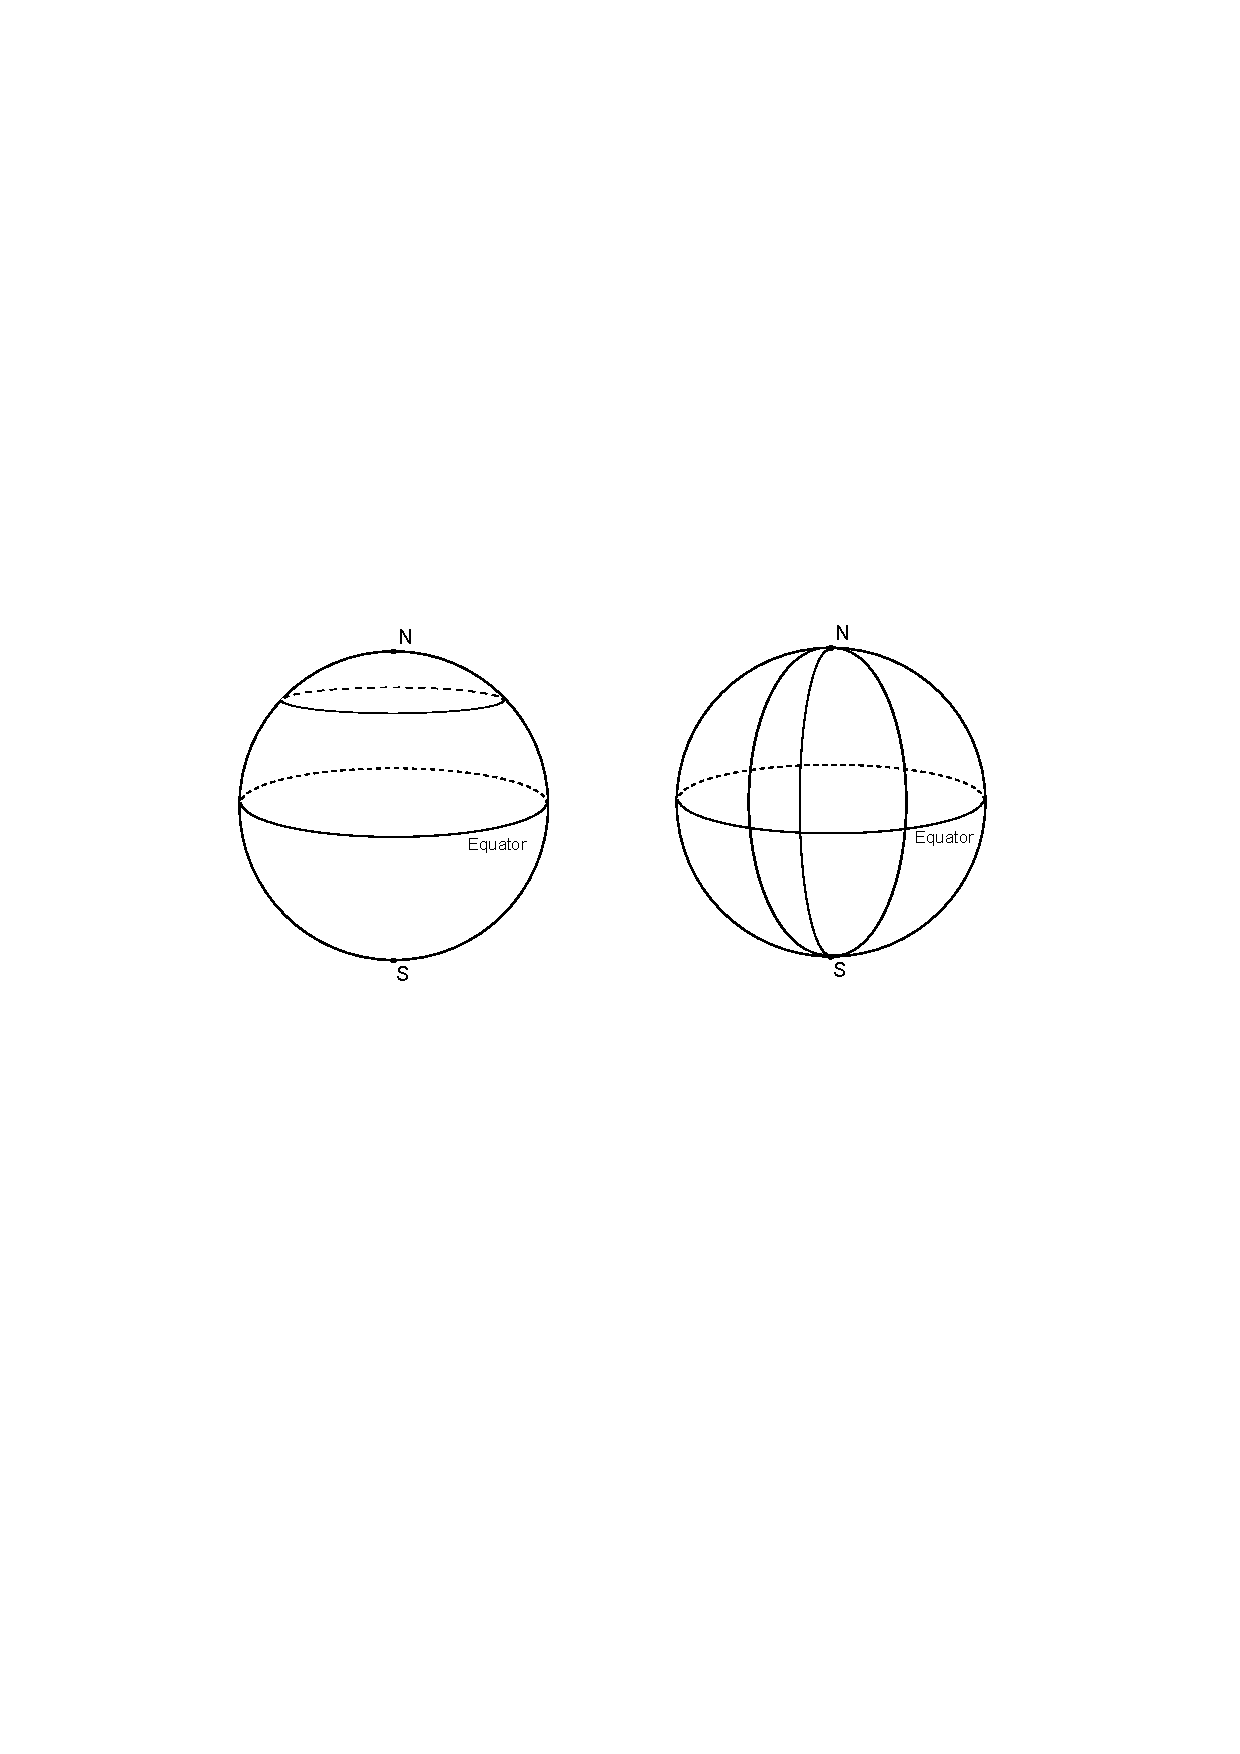
\includegraphics[scale=0.7]{Spherical1}$$
\QM

% Intrinsic vs. extrinsic curvature.  geodesics.  

In non-Euclidean geometries, many familiar results no longer hold.  In spherical geometry, for example, there are no parallel lines because any two lines intersect in two points, and the sum of the angles in a triangle is greater than $180^\circ$.  In hyperbolic geometry, in contrast, parallel lines are not a fixed distance apart, the sum of the angles in a triangle is less than $180^\circ$.  
$$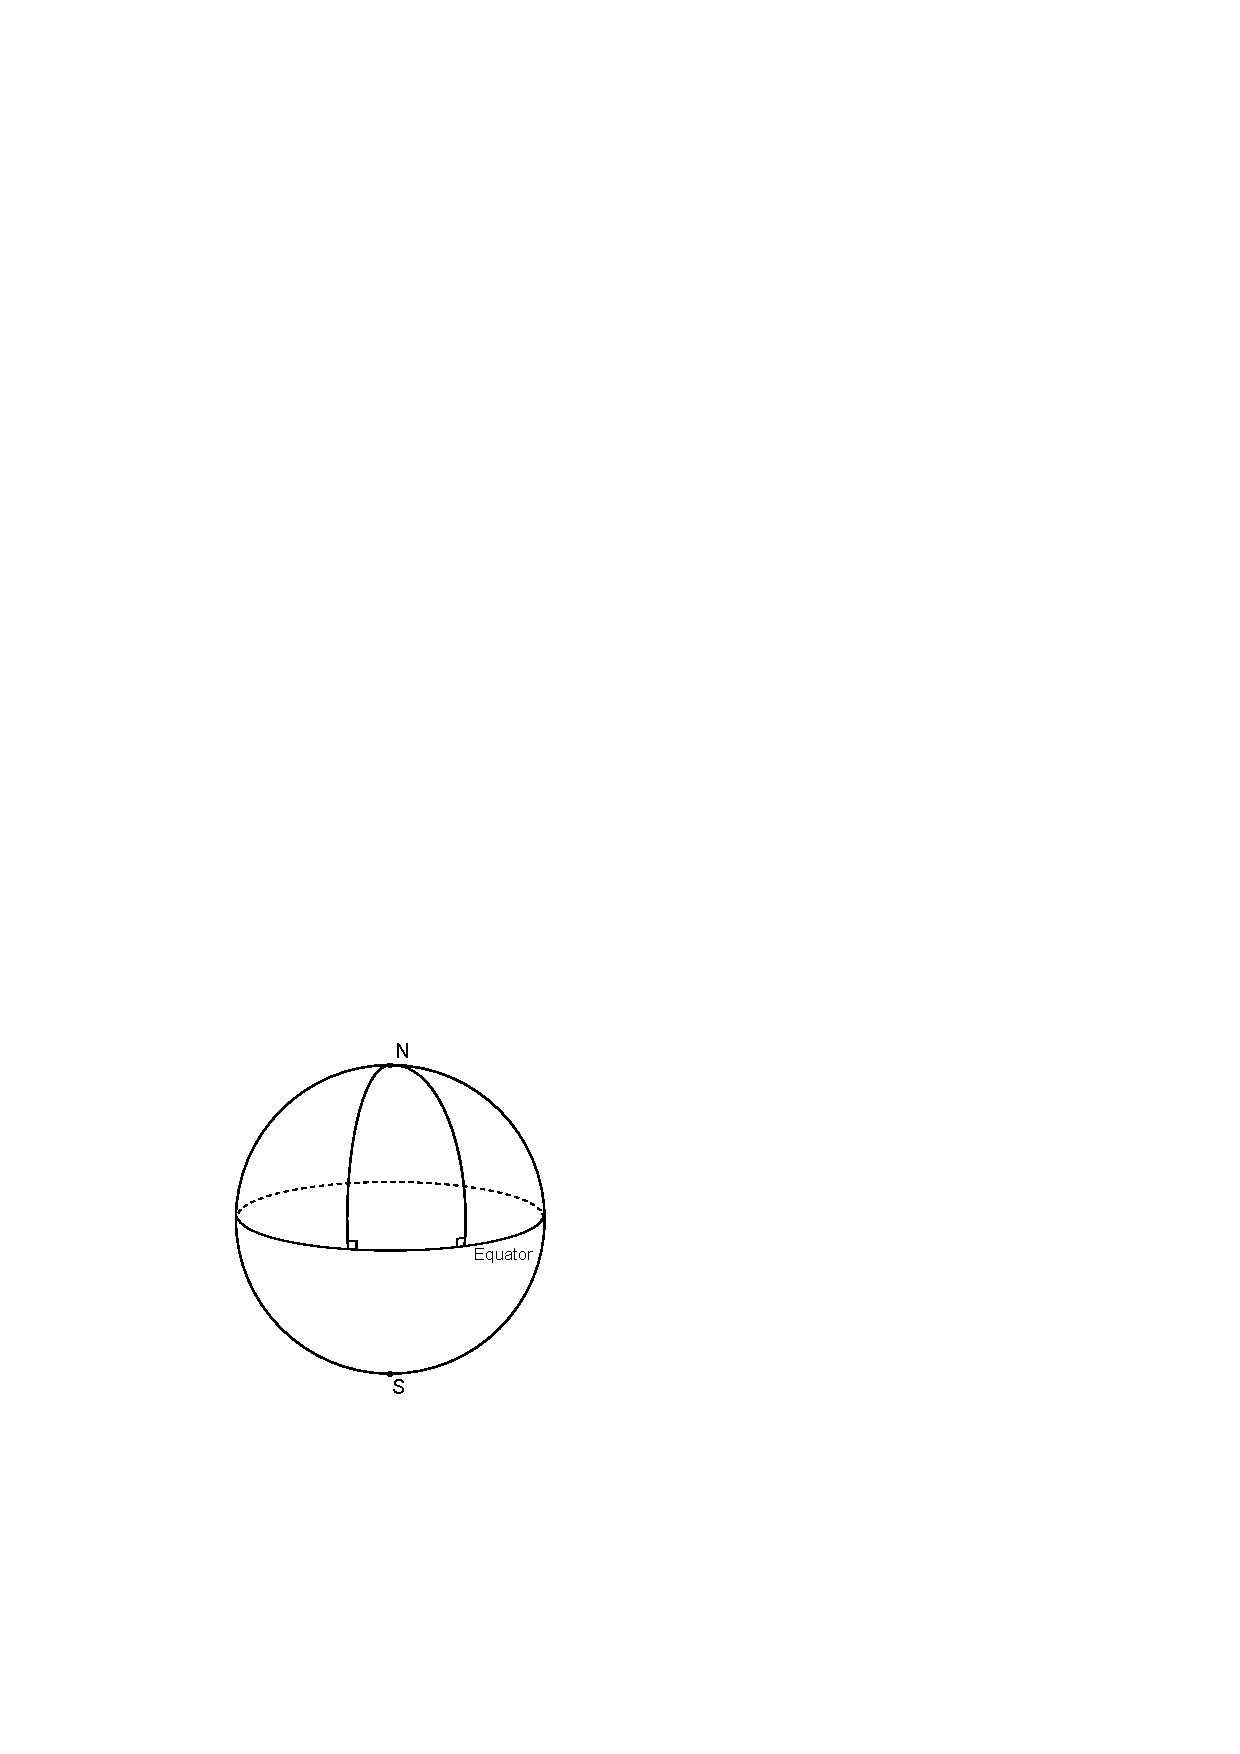
\includegraphics[scale=0.7]{Spherical2}$$

The following statements characterize three different types of geometries:  
\begin{itemize}
\item Euclidean geometry: Given a line and a point not on the line, there is \emph{exactly one line} parallel to the given line.

\item Spherical geometry:  Given a line and a point not on the line, there are \emph{no lines} through the point parallel to the given line. 

\item Hyperbolic geometry:  Given a line and a point not on the line, there is \emph{more than one line} parallel to the given line. 
\end{itemize}

% Each of these geometries requires other postulates, of course.  Here we are merely highlighting a crucial distinction among them.  


In this course, we explore neither spherical nor hyperbolic geometry in detail, but keep these contrasting ideas in mind as we continue to dig into Euclidean geometry.  

\begin{problems}

\begin{enumerate}

\item From the above statements about angle sums in triangles, what can you conclude about angle sums in quadrilaterals  in spherical and hyperbolic geometries?

\item In Euclidean geometry, a rectangle is a quadrilateral with four right angles. 
\begin{enumerate}
\item What can you conclude about rectangles in spherical and hyperbolic geometries?  Explain.  
\item What does this imply about the usefulness of familiar (Euclidean) area formulas in these other geometries?  Explain your reasoning. 
\end{enumerate} 

\item A bear goes traveling.  She walks due south for one mile, turns left $90^\circ$, and walks due east for one mile.  She again turns left $90^\circ$, and then walks due north for one mile, ending in the place where she started.  What color is the bear?  Explain your reasoning.  

\item When walking on a sphere, how could a bug check whether she or he was traveling straight.  

\item In the Euclidean plane, any two distinct points determine a unique line.  Is that true in spherical geometry?  

\item Can the Euclidean definition of a circle make sense on a sphere?  Be sure that the center of the circle is a point on the sphere.  How would you measure the radius of the circle?  

% finding routes of planes or ships on the globe.  Get back to latitude lines. 

% rotations, reflections, and translations on a sphere? 

% Is radius perpendicular to tangent to circle?  

% poles of a great circle  

% perhaps compare area and circumference of the spherical and Euclidean circle.  

%  Problems about symmetries of a line on the sphere.  Use it to argue that great circles are straight.  
% Wrapping a ribbon on a sphere.    
% driving a car with fixed wheels (distance traveled). 


% Betweenness collapses. 
% Two points do not always determine a unique line.  
% antipodal points lie on opposite ends of a diameter
% lines are finite in extent
% perpendicular from a point to a line is not necessarily unique.
% exterior angle theorem 


\end{enumerate}

\end{problems}

\newpage 

\section{Assumptions in Mathematics}
Every area of mathematics is based on a set of assumptions, sometimes called axioms or postulates,\margincomment{In classical mathematics, ``axioms'' were self-evident statements that were common to many areas of science (including mathematics), whereas ``postulates'' were common-sense facts drawn from experience in specific areas, such as geometry.  In modern mathematics, this distinction is no longer seen as significant, and most assumptions are merely called axioms.  In deference to Euclid's \emph{Elements}, the word postulate is used almost exclusively to discuss key assumptions in geometry, as you will see below.}
which are merely statements that are accepted without proof.  They serve as the foundation of the theory being developed, and all other facts are proven beginning with these assumptions.  This approach is called the \emph{axiomatic method}.  

\dots Or at least that's how mathematics is imagined to work.  In practice, because mathematics is so vast and interconnected, most mathematical reasoning and problem solving starts ``in the middle'' from a collection of accepted facts, with little worry about which statements were taken as assumptions and which were proven as theorems.  

And there are choices.  For example, to build Euclidean geometry, we may choose any one of the following statements as an axiom and then prove the other two as theorems:   
\begin{itemize}\parsep0pt\parskip0pt
\item Given a line and a point not on the line, there is \emph{exactly one line} parallel to the given line.
\item If parallel lines are cut by a transversal, then corresponding angles are congruent.
\item The sum of the interior angles of a triangle is $180^\circ$.
\end{itemize}

In these notes, we take the first statement as an axiom, and we prove the other two statements.  

% Incorporate meanings of fractions, and the fundamental assumption of school mathematics.  

\begin{question}
In school mathematics we can ``explain'' the properties of whole or rational numbers by appealing to models and to meanings of the arithmetic operations.  But in advanced mathematics courses, the real numbers are usually specified via axioms, some of the axioms have names.  What are the names of the following axioms:  
\begin{enumerate}
\item $a + b = b + a$  
\item $a(bc) = (ab)c$
\item $a(b+c) = ab + ac$
\item If $a = b$ and $b = c$ then $a = c$ 
\end{enumerate}
\end{question}
\QM

Chances are you used the word ``property'' or ``law'' rather than ``axiom'' in your response.  Some of the properties have important names, such as the \emph{distributive property of multiplication over addition}.  The last of these is called the transitive property of equality.  But in school mathematics, it is neither necessary to instructive to insist that every such property have a shared name.  

% Much of school mathematics proceeds along the same lines:  axioms, assumptions, and postulates are rarely explicit; 
% and outside of the high school geometry course, about the only fact that is called a theorem is that of Pythagoras. 

\subsection{Assumptions for School Geometry}
We propose the following set of assumptions\margincomment{In addition to these geometric assumptions, we of course assume the properties of the algebra of real numbers.} for school geometry:  
{\small
\begin{itemize}
\item[(A1)] Through two distinct points passes a unique line.
\item[(A2)] Given a line and a point not on the line, there is exactly one line passing through the point which is parallel to the given line (Parallel postulate).
\item[(A3)] The points on a line can be placed in one-to-one correspondence with the real numbers so that differences measure distances (Ruler postulate).  
\item[(A4)] The rays with a common endpoint can be numbered so that differences measure angles and so that straight angles measure $180^\circ$ (Protactor postulate). 
\item[(A5)] Every basic rigid motion (rotation, reflection, or translation) has the following properties:
\begin{enumerate}[(i)]\parskip0pt
\item It maps a line to a line, a ray to a ray, and a segment to a segment.
\item It preserves distance and angle measure.
\end{enumerate}
\item [(A6)] Areas of geometric figures have the following properties: 
\begin{enumerate}[(i)]%\parskip0pt\parsep0pt
\item Congruent figures enclose equal areas.
\item Area is additive, i.e., the area of the union of two regions that overlap only at their boundaries is the sum of their areas. 
%\item Area is measured by tiling a region with a two-dimensional unit (such as a square) and parts of the unit, without gaps or overlaps. 
\item A rectangle with side-lengths $a$ and $b$ has area $ab$, where $a$ and $b$ can be any non-negative real numbers.
\end{enumerate}

\end{itemize}
}

\bigskip

These assumptions can be remembered easily in the following chunks:  
\begin{itemize}
\itemsep0em
\item (A1) and (A2):  Points, lines, and parallel lines behave as they should. 
\item (A3) and (A4):  Distance and angle measure behave as they should. 
\item (A5):  Basic rigid motions behave as they should.
\item (A6):  Area behaves as it should.  
\end{itemize}

\begin{question}
Given two distinct lines, if they have no points in common, they are said to be parallel.  Most of the time, of course, they will have exactly one point in common.  Can the two lines have more than one point in common?  Use the above axioms to explain your reasoning.  
\end{question}

%Lemma 2. If three lines L1, L2, and L3 have the property that L1 || L2 and L2 || L3,
%then L1 || L3.

The ruler postulate gives us a definition of betweenness, which allows to to define line segment and ray.    

\begin{definition}
If points $A$, $X$, and $B$ are on a line $l$, we say that $X$ is \emph{between} $A$ and $B$ if $AX + XB = AB$.
\end{definition}

\begin{question}
Use the concept of betweenness to define line segment $\overline{AB}$.  Now use the concept of betweenness to define ray $\overrightarrow{AB}$. 
\end{question}

\begin{question}
Use the protractor postulate to provide a definition of adjacent angles, analogous to betweenness for distances.  
\end{question}

\begin{question}
Prove:  Let $l$ be a line and $O$ be a point on $l$. Let $R$ be the $180^\circ$
rotation around $O$. Then $R$ maps $l$ to to itself.  (Hint:  Pick points $P$ and $Q$ on $l$ so that $O$ is between them, and consider the straight angle $\angle POQ$.)
\end{question}

\begin{theorem}
Let $l$ be a line and $O$ be a point \emph{not} lying on $l$. Let $R$ be the $180^\circ$
rotation around $O$. Then $R$ maps $l$ to a line parallel to itself. 
\end{theorem}

Note:  The following proof uses function notation to describe the images under the rotation $R$.  Thus $R(l)$ is the image of line $l$, and $R(Q)$ is the image of point $Q$.  

\begin{proof}
Suppose $R(l)$ is not parallel to $l$.  Then $R(l)$ and $l$ have a point $Q$ in common.  Because $Q$ is on $R(l)$, there is a point $P$ on $l$, 
so that $R(P) = Q$. Because $R$ is a $180^\circ$ rotation around $O$, the three points $P$, $Q$, and $O$ lie in a line $m$. But
$Q$ is by assumption also a point in $l$, so $l$ and $m$  have two distinct points in common: $P$ and $Q$. 
But $l$ and $R(l)$ are distinct because $O$ is on $m$ but not on $l$. We have a contradiction, and thus $R(l)$ must be parallel to $l$.  
\end{proof}

%Lemma 1 (page 81) and Theorem 1 is proved.
%
%Corollary. Given a line L and point P not on L, there is a line parallel to L and
%passing through P.
%
%Pick Q on L.  Let O be the midpoint of PQ, and use Theorem 1.  
%
%Theorem 2. Two lines perpendicular to the same line are either identical or parallel


\begin{problems}
\begin{enumerate}
\item Use adjacent angles to prove that vertical angles are equal.    
\item Now use rotations to prove that vertical angles are equal.

\item Prove that alternate interior angles and corresponding angles of a transversal with respect to a pair of parallel lines are equal.
\item Prove that the sum of the interior angles of a triangle is $180^\circ$.
\item Prove: If a pair of alternate interior angles or a pair of corresponding angles of a transversal with respect to two lines are equal, then the lines are parallel.
\end{enumerate}
\end{problems}


\section{Dilations, Scaling, and Similarity}
In a previous section, we saw how transformations can be used as a foundation for describing congruence and explaining the triangle congruence criteria.  In this section, we show how transformations can be used to describe similarity.  Because the basic rigid motions all preserve distances, we need a new kind of transformation:  a dilation. 

\begin{definition}
Given a point $O$ and a positive number $r$, a \emph{dilation} about $O$ by scale factor $r$, is a mapping that takes a point $P$ to a point $P'$ so that $OP' = r\cdot OP$.  
\end{definition}

With this definition, rubber bands are natural tools for exploring dilations.  By tying together two rubber bands 
Through explorations with rubber bands and with geometry software, we observe that a dilation has the following properties:\standardhs{G-SRT.1}%\standardhs{G-SRT.1a}\standardhs{G-SRT.1b}  

\begin{enumerate}[(i)]\parskip0pt\parsep0pt
\item It maps lines to lines, rays to rays, and segments to segments.
\item It changes distance by a factor of $r$, where $r$ is the scale factor of the dilation.
\item It maps every line passing through the center of dilation to itself, and it maps every line not passing through the center of the dilation to a parallel line.  
\item It preserves angle measure.
\end{enumerate}

We could assume these properties, just as we have assumed the properties of the basic rigid motions.  It is possible to use our assumptions about area to prove some of these properties.  These are the Side-Splitter Theorems.\standard{8.G.4}  


\begin{definition}
A geometric figure is \emph{similar} to another if the second can be obtained from the first by a sequence of rotations, reflections, translations, and dilations.  
\end{definition}

If the objects are similar, try to find a single dilation that demonstrates the similarity.   If you cannot find such a dilation, explain how you know you cannot.  


\section{Length, Area, and Volume Under Scaling}

\fixnote{To be written.}  

\fixnote{Include problems on making scale drawings and on using scale drawings to solve problems about length and area.}

\fixnote{Also need to write a section for parametric equations, coordinates, functions.}
